\documentclass[conference]{IEEEtran}
\IEEEoverridecommandlockouts
\usepackage{cite}
\usepackage{amsmath,amssymb,amsfonts}
\usepackage{graphicx}
\usepackage{textcomp}
\usepackage{xcolor}
\usepackage{booktabs}
\usepackage{tikz}
\usetikzlibrary{positioning,arrows.meta}
\def\BibTeX{{\rm B\kern-.05em{\sc i\kern-.025em b}\kern-.08em
    T\kern-.1667em\lower.7ex\hbox{E}\kern-.125emX}}
\begin{document}

\title{Association Mining of Cross-Conference Publication Patterns in DBLP: A Temporal Analysis (2015--2025)}

\author{\IEEEauthorblockN{1\textsuperscript{st}Lukas Raja Agripa}
\IEEEauthorblockA{\textit{School of Electrical Engineering and Informatics} \\
\textit{Institut Teknologi Bandung}\\
Bandung, Indonesia \\
lukasagripa27@gmail.com}
\and
\IEEEauthorblockN{2\textsuperscript{nd}Zahran Nizar Fadhlan}
\IEEEauthorblockA{\textit{Faculty of Mechanical and Aerospace Engineering} \\
\textit{Institut Teknologi Bandung}\\
Bandung, Indonesia \\
zahrannizarfadhlan@gmail.com}
}

\maketitle

\begin{abstract}
The DBLP bibliography provides a large-scale view of computer science (CS) publication activity and the venues shared by researchers. This paper mines cross-conference patterns using Apriori and FP-Growth on Author-Based (AB) and Author-Year-Based (AY) transactions, with association rules evaluated at 50\% minimum confidence and temporal analysis across four periods from 2015 to 2025. The cleaned corpus contains 2,000,963 papers, 1,823,008 authors, and 4,494 venues; the mining item universe retains 1,792 venues covering 91.5\% of papers (92.5\% of paper-author rows). NeurIPS ranks first by both paper count and unique authors, and ICML--NeurIPS is the most frequent venue pair. Both algorithms return identical frequent itemsets; FP-Growth is faster at 0.1\% support, whereas Apriori is faster at higher thresholds. The temporal analysis identifies substantial changes in the detected rule set: between 2021--2023 and 2024--2025, 19 rules persist, 300 newly qualify, and 7 are no longer detected at the selected thresholds. Representative later-period rules span artificial intelligence, machine learning, natural language processing, computer vision, and communications. These patterns describe changes in cross-venue publication behavior around the public introduction of ChatGPT, but do not establish that LLMs caused them.
\end{abstract}

\begin{IEEEkeywords}
association rule mining, Apriori, bibliometrics, DBLP, frequent pattern mining, FP-Growth
\end{IEEEkeywords}

\section{Introduction}
In computer science (CS), conferences rather than journals are the primary venue for new results, and the DBLP bibliography \cite{dblp} indexes millions of such papers. The sheer volume makes it hard to see which conferences matter most to the community and which ones share the same researchers.

The rapid development and increasing public visibility of LLMs provide a timely context for examining changes in computer science (CS) publication activity. The emergence and widespread adoption of LLMs technologies around 2022 marked a significant development in the research and academic landscape. This period falls within our 2021–2023 interval, while 2024–2025 represents the first complete interval following the broader emergence of these technologies. We therefore examine how cross-conference publication rules evolve across the prescribed periods and interpret the subsequent patterns within this broader technological context, without treating temporal coincidence as evidence of causation.

We measure popularity by publication activity and discover relations between conferences with frequent pattern mining and association rules, using Apriori \cite{apriori} and FP-Growth \cite{fpgrowth}. Each transaction is the set of venues an author published in, and a rule $X \Rightarrow Y$ says that authors of $X$ tend to also publish in $Y$.

The contributions of this paper are:
\begin{itemize}
\item A reproducible DBLP preprocessing pipeline for 2015--2025 conference papers (2,000,963 papers after cleaning).
\item A comparison of two transaction models, Author-Based (AB) and Author-Year-Based (AY).
\item An evaluation of Apriori and FP-Growth, both implemented from scratch and validated against the mlxtend library.
\item A temporal analysis that identifies persistent, newly qualifying, and no-longer-detected rules across four periods, followed by an interpretation of the CS areas represented by the venues involved.
\end{itemize}

This paper answers five research questions:
\begin{itemize}
\item RQ1: Which conferences are the most popular by number of papers and by number of unique authors, and do the rankings agree?
\item RQ2: Which conference combinations occur together most often, and which rules have the highest lift?
\item RQ3: Do the AB and AY models produce different patterns?
\item RQ4: Is Apriori or FP-Growth more suitable for DBLP?
\item RQ5: How do conference association rules vary across the four periods from 2015 to 2025, and what patterns are observed around the rise of LLMs?
\end{itemize}

Section~II reviews related work, Section~III describes the dataset, Section~IV the methodology, Section~V the experimental setup, Section~VI the results, Section~VII the limitations, and Section~VIII concludes.

\section{Related Work}
\textbf{Frequent pattern mining.} Apriori \cite{apriori} finds frequent itemsets level by level and prunes candidates with the anti-monotone property of support. FP-Growth \cite{fpgrowth} avoids candidate generation by compressing the data into a prefix tree and mining conditional pattern bases. We implement both and compare them on the same data.

\textbf{Bibliometrics on DBLP.} Prior work analyzed DBLP from the angle of authors and communities. Kim \cite{kim} studied computer scientists who publish in both conferences and journals and found that conference papers form a distinct channel of scholarly communication. Biryukov and Dong \cite{biryukov} traced researcher careers and compared CS communities by productivity and stability. K\"ull \cite{kull} analyzed about five million DBLP publications for trends in volume, topics and the conference-journal balance. Schommer \cite{schommer} proposed a descriptive framework for typifying social communities in DBLP.

\textbf{Positioning.} These studies provide complementary views of DBLP through author productivity, collaboration, and community structure. We take a transaction-based view in which each author's set of publication venues is treated as an itemset, allowing recurring cross-venue combinations and association rules to be examined directly. The author-year representation adds a time-local view of these combinations, while the temporal analysis compares their prevalence across four periods.

\section{Dataset}
We use the full DBLP XML release \cite{dblp} and keep only \texttt{inproceedings} records whose DBLP year field falls between 2015 and 2025. When this field differs from the year in the proceedings cross-reference, we consistently retain the record-level DBLP year. Each record has a unique key, the venue is usually implied in the key (\texttt{conf/<venue>/...}), and authors with identical names may be distinguished by a numeric suffix assigned by DBLP. Table~\ref{tab:dataset} summarizes the data.

\begin{table}[t]
\caption{Dataset Description}
\label{tab:dataset}
\centering
\footnotesize
\begin{tabular}{p{2.3cm}p{5.1cm}}
\toprule
Item & Value \\
\midrule
Source & dblp.xml.gz from dblp.org \cite{dblp} \\
Retrieval date & 23 Nov 2026 (00:21 UTC); file modified 20 Nov 2026 \\
File size & 1,123,383,693 bytes (gz); 5.42 GB uncompressed \\
SHA-256 & 7f428224...715a47ce5 \\
All records & 13,135,541 \\
Main record types & article 4,531,934; www 4,249,796; inproceedings 4,004,881; phdthesis 158,395; incollection 71,264; proceedings 65,917 \\
Attributes used & author, title, year, booktitle, key, crossref \\
Raw 2015--2025 & 2,004,427 inproceedings \\
After cleaning & 2,000,963 papers; 1,823,008 authors; 4,494 venues \\
\bottomrule
\end{tabular}
\end{table}

\section{Methodology}
Fig.~\ref{fig:pipeline} shows the pipeline.

\begin{figure}[t]
\centering
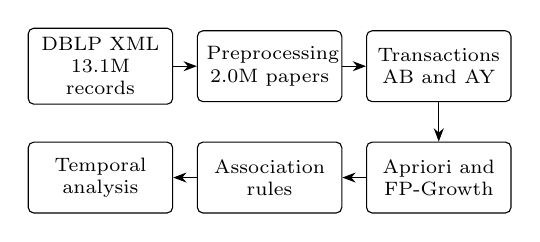
\begin{tikzpicture}[box/.style={draw,rounded corners=2pt,font=\scriptsize,align=center,minimum height=0.9cm,text width=1.6cm},>=Stealth]
\node[box] (a) {DBLP XML\\13.1M records};
\node[box,right=0.3cm of a] (b) {Preprocessing\\2.0M papers};
\node[box,right=0.3cm of b] (c) {Transactions\\AB and AY};
\node[box,below=0.5cm of c] (d) {Apriori and\\FP-Growth};
\node[box,left=0.3cm of d] (e) {Association\\rules};
\node[box,left=0.3cm of e] (f) {Temporal\\analysis};
\draw[->] (a)--(b); \draw[->] (b)--(c); \draw[->] (c)--(d); \draw[->] (d)--(e); \draw[->] (e)--(f);
\end{tikzpicture}
\caption{Overview of the mining pipeline.}
\label{fig:pipeline}
\end{figure}

\subsection{Preprocessing}
We parse the XML in a streaming fashion and keep \texttt{inproceedings} from 2015 to 2025. We (1) remove records missing a key, title, year, or author (2,255 records); (2) retain valid years in the observation period; and (3) remove front matter such as prefaces (1 record). For venue normalization, we prefer the venue segment of the DBLP key because \texttt{booktitle} has inconsistent spellings (up to 165 variants for MICCAI); \texttt{booktitle} is used as a fallback when the key does not encode a conference venue, and the NIPS alias is merged into NeurIPS. Author strings are normalized with Unicode NFKC and whitespace cleanup, while DBLP disambiguation suffixes are retained to avoid merging homonymous authors. Finally, we remove duplicate keys and apply a secondary content signature based on title, year, venue, and author set (1,208 additional records).

\subsection{Transactional Databases}
Let $V$ be the set of venues used as items. In the AB model, one transaction per author contains the distinct venues at which that author published during 2015--2025. In the AY model, one transaction represents an (author, year) pair and contains the distinct venues in which that author published in that year. We retain venues with at least 200 papers as items, reducing the total items from 4,494 to 1,792 venues while retaining 91.5\% of papers, 92.5\% of paper-author rows, and 93.9\% of authors. This threshold represents a practical balance between data coverage and computational tractability rather than an indicator of venue quality. An AB transaction is created only for an author with at least one retained venue, and an AY transaction only for an author-year pair with at least one retained venue. Thus, support is calculated over the eligible transaction population (1,711,805 AB transactions or 3,826,978 AY transactions), not over all author names in the cleaned corpus. Single-item transactions remain in the database and in the support denominator, although they cannot form multi-venue itemsets or rules.

\subsection{Apriori}
Apriori generates candidate $k$-itemsets from frequent $(k-1)$-itemsets and prunes any candidate with an infrequent subset. Our implementation counts support with vertical bitsets, with join and prune steps. It was checked against mlxtend on a 50,000-transaction sample at 1\% support, where itemsets and supports were identical.

\subsection{FP-Growth}
Transactions are inserted into an FP-tree ordered by item frequency. Mining proceeds recursively over conditional pattern bases, so no candidate itemsets are generated. Our own implementation was validated against mlxtend in the same test.

\subsection{Association Rules}
With $D$ the set of transactions and $X$, $Y$ sets of venues,
\begin{align}
\mathrm{supp}(X) &= \frac{|\{T\in D : X\subseteq T\}|}{|D|},\\
\mathrm{conf}(X\Rightarrow Y) &= \frac{\mathrm{supp}(X\cup Y)}{\mathrm{supp}(X)},\\
\mathrm{lift}(X\Rightarrow Y) &= \frac{\mathrm{conf}(X\Rightarrow Y)}{\mathrm{supp}(Y)}.
\end{align}
Here, $D$ denotes the relevant transaction database (AB, AY, or a period-specific AY subset). Rules are generated from every frequent itemset with a minimum confidence of 50\%. We rank rules by lift: a value above 1 indicates that $X$ and $Y$ co-occur more frequently than expected under statistical independence.

\subsection{Temporal Analysis}
We split the AY database into 2015--2017, 2018--2020, 2021--2023, and 2024--2025 and mine each period independently using FP-Growth. A common relative minimum support of 0.05\% and minimum confidence of 50\% are applied in every period. Rules are compared between consecutive periods using their exact antecedent and consequent: a rule is persistent if it qualifies in both periods, newly qualifying if it qualifies only in the later period, and no longer detected if it qualifies only in the earlier period. A rule not detected in a period may still occur below the selected support or confidence thresholds. After mining, representative rules are interpreted by the broad research areas of their venues. The ACM Computing Classification System provides a general vocabulary for these area labels \cite{acmccs}; venue assignments are based on primary scope and are descriptive, not constraints on mining. Interdisciplinary venues may represent more than one area. The 2021--2023 interval includes the emergence and growing public adoption of LLMs, so it is treated as a transition period rather than a purely pre-LLM baseline.

\section{Experimental Setup}
Table~\ref{tab:params} lists the parameters needed to reproduce the experiments.

\begin{table}[t]
\caption{Experimental Parameters}
\label{tab:params}
\centering
\footnotesize
\begin{tabular}{p{2.4cm}p{5.0cm}}
\toprule
Parameter & Value \\
\midrule
Environment & Google Colab, Python 3.13, lxml, pandas, NumPy, pyarrow, mlxtend \\
DBLP release & Downloaded 23 Nov 2026 \\
Data period & 2015--2025 \\
Item threshold & 200 papers per venue (1,792 of 4,494 venues; 92.5\% of paper-author rows) \\
Minimum support & 0.1\%, 0.5\%, 1\%, 2\% \\
Minimum confidence & 50\% \\
Metrics & Number of itemsets and rules; execution time as an additional measure \\
Random seed & 42 \\
Temporal periods & 2015--2017, 2018--2020, 2021--2023, 2024--2025 \\
Temporal support & 0.05\% of transactions in each period (AY) \\
\bottomrule
\end{tabular}
\end{table}

\section{Results and Discussion}
\subsection{Preprocessing Results}
The raw data was overall already clean: preprocessing left 2,000,963 of 2,004,427 papers (99.8\%). Some 2,666 records carry a year that differs from the proceedings year, and we kept the DBLP year field. Papers per year grow from 161,287 in 2015 to 213,692 in 2024. The venue distribution has a long tail: 4,494 venues exist, but the 1,792 venues with at least 200 papers already cover 91.5\% of all papers.

\subsection{Conference Popularity (RQ1)}
NeurIPS ranks first by papers (25,455) and by unique authors (57,801), so the top rank agrees across both measures (Table~\ref{tab:top10}). Eight of the top ten venues appear in both rankings, and the Spearman correlation between the two rankings is 0.987 over all venues and 0.857 over the top 50. The rankings differ for some venues: AAAI is sixth by papers but third by authors, and ICC is tenth by papers but nineteenth by authors. Growth is uneven (Fig.~\ref{fig:trend}): NeurIPS grows 13.2 times from 440 papers in 2015 to 5,823 in 2025 and EMNLP 10.8 times, while all papers grow only 1.24 times. IGARSS and EMBC show zero papers in 2025, most likely because they were not yet indexed in the release we used, so their 2025 counts should be read with care.

\begin{table}[t]
\caption{Top-10 Venues by Paper Count and Unique Authors}
\label{tab:top10}
\centering
\footnotesize
\begin{tabular}{rlrlr}
\toprule
Rank & By papers & Papers & By authors & Authors \\
\midrule
1 & NeurIPS & 25,455 & NeurIPS & 57,801 \\
2 & CVPR & 22,752 & CVPR & 47,664 \\
3 & ICASSP & 21,606 & AAAI & 46,434 \\
4 & HCI & 19,912 & ICASSP & 42,060 \\
5 & IGARSS & 19,685 & EMBC & 39,319 \\
6 & AAAI & 19,276 & HCI & 37,884 \\
7 & CHI & 14,834 & IGARSS & 35,229 \\
8 & EMNLP & 14,814 & EMNLP & 33,957 \\
9 & EMBC & 14,677 & ICML & 31,896 \\
10 & ICC & 14,329 & ICLR & 31,315 \\
\bottomrule
\end{tabular}
\end{table}

\begin{figure}[t]
\centering
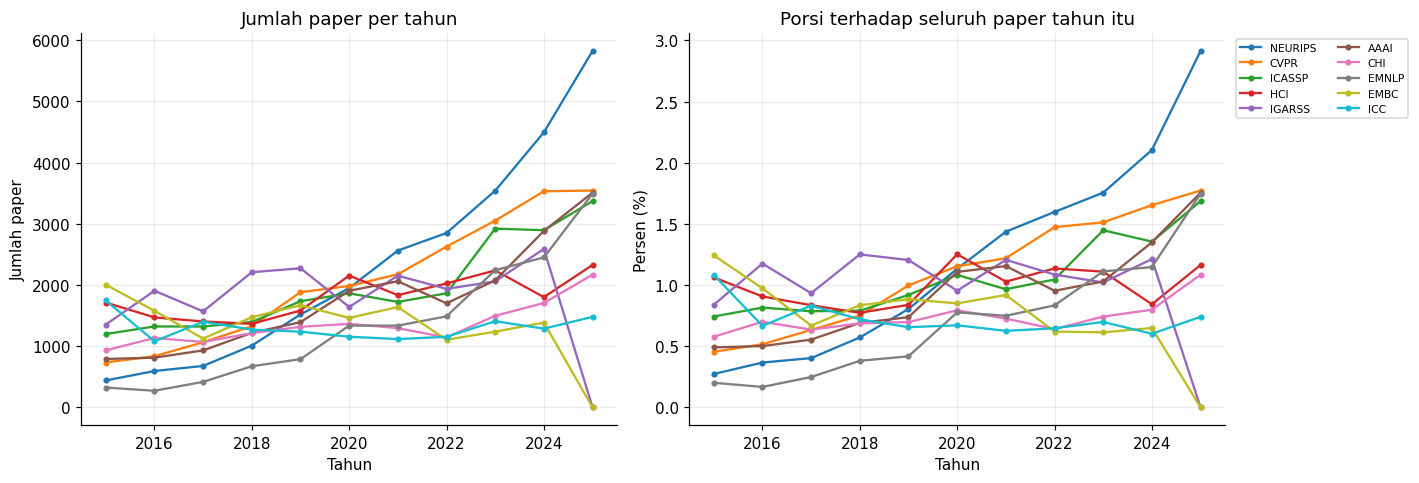
\includegraphics[width=\columnwidth]{fig_trend.png}
\caption{Papers per year (left) and share of all papers in that year (right) for the ten venues with the most papers.}
\label{fig:trend}
\end{figure}

\subsection{Transactional Databases (RQ3)}
The AB database contains 1,711,805 eligible-author transactions, while the AY database contains 3,826,978 eligible author-year transactions. Both use the same 1,792-venue item universe. AB has an average of 2.57 venues per transaction, compared with 1.56 for AY. Single-venue transactions account for 59.0\% of AB and 71.8\% of AY; consequently, 702,200 AB and 1,080,973 AY transactions contain at least two venues and can contribute to multi-venue patterns. AB captures an author's venue history across the full period (18.1 million venue pairs and up to 289 venues in one transaction), whereas AY captures same-year activity but gives authors with publications in multiple years more than one transaction (2.24 transactions per represented author on average).

\subsection{Frequent Patterns}
The number of frequent itemsets falls quickly as minimum support rises (Table~\ref{tab:itemsets}). At 2\% only seven single venues remain; pairs appear at 1\% or lower and triples only at 0.5\% or lower (ICLR, ICML, and NeurIPS). The ten most frequent singleton itemsets correspond to the leading venues by unique authors in Table~\ref{tab:top10}; Table~\ref{tab:pairs} lists the ten most frequent multi-venue itemsets at 0.1\% support. The leading pair is ICML--NeurIPS, present in 18,502 eligible-author transactions (1.081\%); other frequent pairs connect venues in machine learning, computer vision, language, and robotics. The repeated appearance of venues from related areas suggests that the mining captures recognizable publication communities, while the pair frequencies measure co-publication rather than venue quality.

\begin{table}[t]
\caption{Top-10 Multi-Venue Itemsets (AB, 0.1\% Support)}
\label{tab:pairs}
\centering
\footnotesize
\begin{tabular}{lrr}
\toprule
Venue pair & Transactions & Support (\%) \\
\midrule
ICML + NeurIPS & 18,502 & 1.081 \\
ICLR + NeurIPS & 17,910 & 1.046 \\
AAAI + NeurIPS & 15,971 & 0.933 \\
CVPR + NeurIPS & 15,634 & 0.913 \\
CVPR + ICCV & 15,439 & 0.902 \\
ACL + EMNLP & 14,558 & 0.850 \\
CVPR + ECCV & 13,752 & 0.803 \\
ICLR + ICML & 12,991 & 0.759 \\
AAAI + CVPR & 12,166 & 0.711 \\
ICRA + IROS & 11,858 & 0.693 \\
\bottomrule
\end{tabular}
\end{table}

\begin{table}[t]
\caption{Frequent Itemsets by Minimum Support (AB)}
\label{tab:itemsets}
\centering
\footnotesize
\begin{tabular}{lrrrr}
\toprule
Itemset size & 0.1\% & 0.5\% & 1\% & 2\% \\
\midrule
1-itemsets & 623 & 76 & 31 & 7 \\
2-itemsets & 439 & 23 & 2 & 0 \\
3-itemsets & 391 & 1 & 0 & 0 \\
4 or more & 243 & 0 & 0 & 0 \\
Total & 1,696 & 100 & 33 & 7 \\
\bottomrule
\end{tabular}
\end{table}

\subsection{Association Rules (RQ2)}
At 0.1\% support and 50\% confidence, the AB database yields 1,614 rules with lift values from 14.9 to 162 (median 33.6). Values above 1 indicate positive association relative to the independence baseline; they do not imply that the venues are rare or unlikely to co-occur. The highest-lift rule links ECCV, MM, and NeurIPS to AAAI, CVPR, and ICCV (lift 162, confidence 0.613), indicating a group of authors publishing across several vision and machine-learning venues (Table~\ref{tab:rules}). For single-venue-to-single-venue rules, the highest lifts are ECOC $\Rightarrow$ OFC (75.3, optical communications), ASRU $\Rightarrow$ INTERSPEECH (69.7, speech), and EACL $\Rightarrow$ ACL (34.4, language).

High support does not mean high lift (Fig.~\ref{fig:lift}). ICML $\Rightarrow$ NeurIPS has the highest support (1.08\%) but a lift of only 17.2, while ECOC $\Rightarrow$ OFC has a support of 0.26\% and a lift of 75.3. The Spearman correlation between rule support and lift is $-0.194$, and between consequent support and lift it is $-0.913$, so rare consequents tend to give large lift. Support measures how many authors follow a pattern, confidence the chance that an author of $X$ also publishes in $Y$, and lift how much stronger that is than chance.

\begin{table*}[t]
\caption{Top-10 Association Rules by Lift (AB, 0.1\% Minimum Support, 50\% Minimum Confidence)}
\label{tab:rules}
\centering
\scriptsize
\setlength{\tabcolsep}{3pt}
\begin{tabular}{p{3.15cm}p{3.15cm}rrr}
\toprule
Antecedent & Consequent & Support (\%) & Confidence & Lift \\
\midrule
ECCV, MM, NeurIPS & AAAI, CVPR, ICCV & 0.1067 & 0.6129 & 162.1 \\
CVPR, ECCV, ICML & ICCV, ICLR, NeurIPS & 0.1080 & 0.5024 & 160.9 \\
CVPR, ICCV, ICML, NeurIPS & ECCV, ICLR & 0.1080 & 0.5138 & 149.0 \\
CVPR, ECCV, ICML, NeurIPS & ICCV, ICLR & 0.1080 & 0.5913 & 147.1 \\
ECCV, ICCV, ICML & CVPR, ICLR, NeurIPS & 0.1080 & 0.6139 & 146.2 \\
ICLR, NAACL & ACL, EMNLP, NeurIPS & 0.1121 & 0.5018 & 142.7 \\
CVPR, ICCV, MM, NeurIPS & AAAI, ECCV & 0.1067 & 0.5753 & 138.8 \\
EMNLP, NAACL, NeurIPS & ACL, ICLR & 0.1121 & 0.5463 & 137.1 \\
CVPR, ECCV, MM, NeurIPS & AAAI, ICCV & 0.1067 & 0.6850 & 136.8 \\
ECCV, ICCV, ICML & AAAI, CVPR, NeurIPS & 0.1012 & 0.5754 & 135.0 \\
\bottomrule
\end{tabular}
\end{table*}

\begin{figure}[t]
\centering
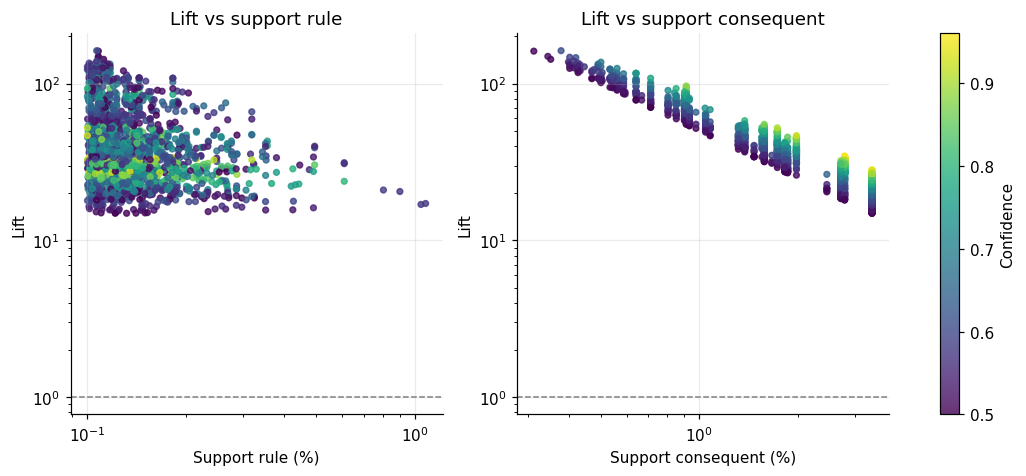
\includegraphics[width=\columnwidth]{fig_lift.png}
\caption{Lift against rule support (left) and against consequent support (right); color shows confidence.}
\label{fig:lift}
\end{figure}

\subsection{Author-Based versus Author-Year-Based (RQ3)}
At a 0.1\% relative minimum support, AB yields 1,696 itemsets and 1,614 rules, while AY yields 380 itemsets and 3 rules (Table~\ref{tab:abay}). Although the highest-support venue pairs are largely consistent between the two models, with 18 of the top 20 pairs appearing in both, the overlap in association rules is limited (Jaccard similarity of 0.002), with only three shared rules exhibiting the same lift order. The difference follows from the transaction units: AB aggregates each author's venues over the full period, while AY requires venues to occur within the same author-year transaction. The two models describe complementary long-term and year-specific patterns rather than competing estimates of the same quantity.

\subsection{Algorithm Comparison (RQ4)}
Apriori and FP-Growth return identical frequent itemsets at every tested minimum support, and both match mlxtend on a 50,000-transaction validation sample (Table~\ref{tab:algo}). Lowering support increases the number of itemsets and rules sharply: 1,614 rules are produced at 0.1\% support, compared with 7 at 0.5\%. Runtime depends on the implementation: our bitset-based Apriori is slower at 0.1\% (17.73 s versus 10.96 s), where many itemsets are generated, while it is faster at higher thresholds (0.06--0.56 s versus 0.53--2.15 s) (Fig.~\ref{fig:runtime}). Thus, neither algorithm is uniformly faster: FP-Growth is advantageous at the lowest tested support, whereas Apriori is more efficient at the higher thresholds in this implementation.

\begin{table}[t]
\caption{Apriori versus FP-Growth (AB)}
\label{tab:algo}
\centering
\footnotesize
\begin{tabular}{lrrrr}
\toprule
Min. supp. & Itemsets & Rules & Apriori (s) & FP-Growth (s) \\
\midrule
0.1\% & 1,696 & 1,614 & 17.73 & 10.96 \\
0.5\% & 100 & 7 & 0.56 & 2.15 \\
1\% & 33 & 2 & 0.11 & 0.93 \\
2\% & 7 & 0 & 0.06 & 0.53 \\
\bottomrule
\end{tabular}
\end{table}

\begin{figure}[t]
\centering
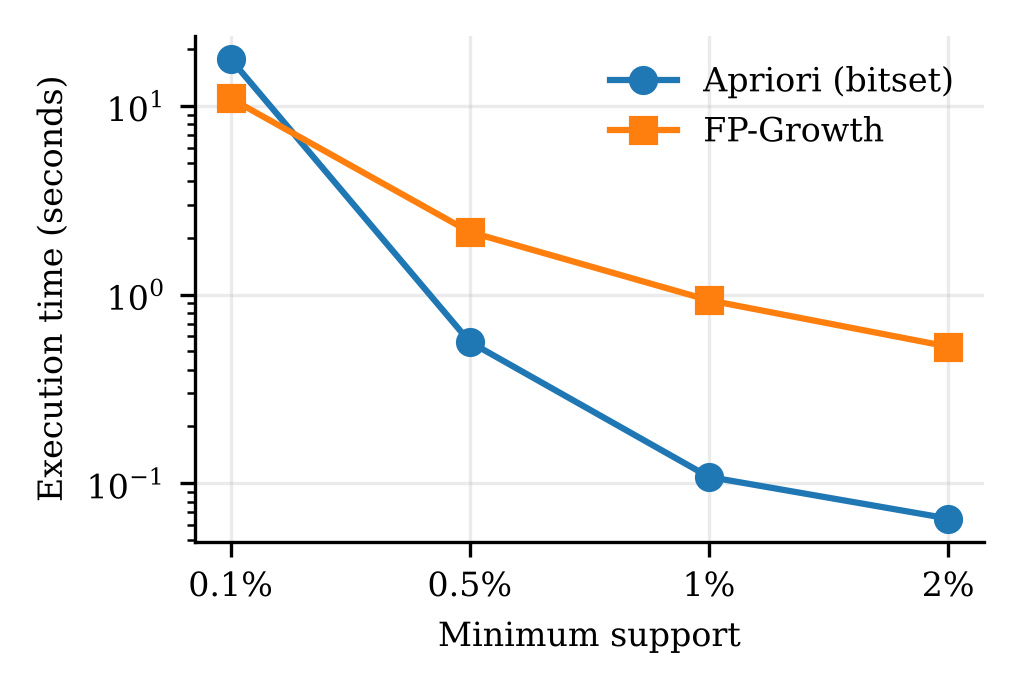
\includegraphics[width=0.85\columnwidth]{fig_runtime.png}
\caption{Execution time of Apriori and FP-Growth against minimum support (log scale).}
\label{fig:runtime}
\end{figure}

\subsection{Temporal Analysis (RQ5)}
Multi-venue patterns become more numerous in the later periods (Table~\ref{tab:temporal}). Frequent pairs increase from 52 in 2015--2017 to 305 in 2024--2025, triples from 2 to 227, and 97 itemsets with four or more venues appear in the final period. The number of association rules rises from 2 to 319. We compare the rule sets between consecutive periods to distinguish persistent, newly qualifying, and no-longer-detected rules (Table~\ref{tab:ruletrans}). No rule persists from 2015--2017 to 2018--2020; three persist from 2018--2020 to 2021--2023; and 19 persist from 2021--2023 to 2024--2025. In the last transition, 300 rules newly qualify and 7 are no longer detected. No rule is present in all four periods.

The venue combinations in the highest-lift rules span several areas of computer science rather than a single predefined grouping. Table~\ref{tab:periodrules} gives one leading example from each period. The 2015--2017 rule ECOC $\Rightarrow$ OFC represents optical communications. In 2018--2020, AAAI and ACL $\Rightarrow$ EMNLP links general artificial intelligence and natural language processing. The leading 2021--2023 rule, SLT $\Rightarrow$ INTERSPEECH, represents speech and language technology. In 2024--2025, AAAI, EMNLP, and ICLR $\Rightarrow$ ACL and NeurIPS spans AI, NLP, and machine learning. Another high-lift rule in the final period links ICCV, ICLR, and ICML to CVPR and NeurIPS (lift 60.2), combining computer vision and machine learning.

The changes are not exclusively associated with AI-related venues. For example, ICC and WCNC $\Rightarrow$ GLOBECOM is detected in both 2018--2020 and 2024--2025 (lifts 45.6 and 48.3), but not in the intervening period. This reappearance shows that some venue associations can recur after temporarily falling below the mining thresholds. Overall, the later rules represent a wider range of cross-venue combinations, including communications, speech, language, AI/ML, and vision.

\begin{table}[t]
\caption{Itemsets and Rules per Period (AY, 0.05\% Support)}
\label{tab:temporal}
\centering
\footnotesize
\begin{tabular}{lrrrr}
\toprule
Measure & 15--17 & 18--20 & 21--23 & 24--25 \\
\midrule
Transactions (thousands) & 855 & 1,014 & 1,121 & 837 \\
Frequent itemsets & 910 & 868 & 926 & 1,267 \\
2-itemsets & 52 & 91 & 148 & 305 \\
3-itemsets & 2 & 6 & 31 & 227 \\
4 or more & 0 & 0 & 0 & 97 \\
Rules & 2 & 5 & 26 & 319 \\
\bottomrule
\end{tabular}
\end{table}

\begin{table}[t]
\caption{Rule Changes Between Consecutive Periods (AY, 0.05\% Support)}
\label{tab:ruletrans}
\centering
\footnotesize
\begin{tabular}{lrrrr}
\toprule
Transition & Persistent & New & Lost & Jaccard \\
\midrule
15--17 $\rightarrow$ 18--20 & 0 & 5 & 2 & 0.000 \\
18--20 $\rightarrow$ 21--23 & 3 & 23 & 2 & 0.107 \\
21--23 $\rightarrow$ 24--25 & 19 & 300 & 7 & 0.058 \\
\bottomrule
\end{tabular}
\end{table}

\begin{table*}[t]
\caption{Representative Highest-Lift Rule in Each Period and Its Main Research Area}
\label{tab:periodrules}
\centering
\scriptsize
\setlength{\tabcolsep}{4pt}
\begin{tabular}{p{1.35cm}p{6.1cm}rrrp{4.3cm}}
\toprule
Period & Rule & Support (\%) & Confidence & Lift & Main area represented \\
\midrule
2015--2017 & ECOC $\Rightarrow$ OFC & 0.20 & 0.516 & 55.4 & Optical communications \\
2018--2020 & AAAI, ACL $\Rightarrow$ EMNLP & 0.06 & 0.582 & 67.5 & Artificial intelligence and NLP \\
2021--2023 & SLT $\Rightarrow$ INTERSPEECH & 0.05 & 0.502 & 52.8 & Speech and language technology \\
2024--2025 & AAAI, EMNLP, ICLR $\Rightarrow$ ACL, NeurIPS & 0.06 & 0.520 & 86.1 & AI, NLP, and machine learning \\
\bottomrule
\end{tabular}
\end{table*}

The rule comparisons are threshold-dependent: a rule classified as newly qualifying may have occurred previously but remained below the minimum support or confidence. The first two periods also yield few rules, limiting rule-level comparisons. Finally, 2024--2025 covers only two years, and some 2025 records may not yet be indexed. LLM's public introduction falls within 2021--2023 period; therefore, this period is treated as a transition period rather than post/pre-LLM period. The observed venue associations are descriptive and cannot establish that LLMs caused the temporal changes.

\begin{table}[t]
\caption{Author-Based versus Author-Year-Based (Same Minimum Support)}
\label{tab:abay}
\centering
\footnotesize
\begin{tabular}{lrr}
\toprule
Measure & AB & AY \\
\midrule
Transactions & 1,711,805 & 3,826,978 \\
Unique venue items & 1,792 & 1,792 \\
Average items per transaction & 2.571 & 1.563 \\
Maximum items per transaction & 289 & 75 \\
Frequent itemsets & 1,696 & 380 \\
Itemsets with 2+ venues & 1,073 & 53 \\
Rules & 1,614 & 3 \\
Top rule lift & 162.1 & 25.4 \\
\bottomrule
\end{tabular}
\end{table}

\section{Limitations and Threats to Validity}
The results should be interpreted within several limits. Popularity measures publication activity rather than research quality or citation impact, and DBLP author disambiguation and metadata-based deduplication may still leave merged, split, or duplicate records. The 200-paper item threshold retains 91.5\% of papers but underrepresents smaller venues. Authors and author-year pairs with no retained venue are omitted, so support is conditional on the eligible transaction populations. AB and AY have different observational units. Temporal rule changes are sensitive to the selected support and confidence thresholds; a rule not detected in a period is not necessarily absent from the underlying publication activity. The early periods yield few rules, and 2024--2025 covers only two years with potentially incomplete 2025 indexing. Venue-to-field labels are interpretive because conference scopes can overlap. Finally, the 2021--2023 interval straddles the public introduction of LLMs, and the observational associations do not establish that LLMs caused the changes.

\section{Conclusion}
NeurIPS ranks first by both paper count (25,455) and unique authors (57,801), and ICML--NeurIPS is the most frequent venue pair. The highest lifts, however, occur in more specialized associations, confirming that publication popularity does not imply the strongest association. AB captures long-term author venue histories, while AY captures same-year behavior. Apriori and FP-Growth return identical itemsets, although their runtime depends on the support threshold. The temporal analysis shows substantial turnover in qualifying rules: from 2021--2023 to 2024--2025, 300 rules newly qualify, 19 persist, and 7 are no longer detected. Representative rules span communications, speech and language technology, AI, NLP, machine learning, and computer vision. These changes coincide with the period following ChatGPT's public introduction, but the study cannot attribute them to LLMs. Future work includes lower-support robustness checks, citation-weighted associations, journal publications, paper-level topic analysis, more complete 2025 data, and sequential temporal rules.

\section*{Acknowledgment}
The authors thank the DBLP team at Schloss Dagstuhl and the University of Trier for providing the data.

\begin{thebibliography}{00}
\bibitem{dblp} ``DBLP computer science bibliography,'' Schloss Dagstuhl and University of Trier. [Online]. Available: https://dblp.org/. Accessed: Nov. 23, 2026.
\bibitem{apriori} R. Agrawal and R. Srikant, ``Fast algorithms for mining association rules,'' in \textit{Proc. 20th Int. Conf. Very Large Data Bases (VLDB)}, 1994, pp. 487--499.
\bibitem{fpgrowth} J. Han, J. Pei, and Y. Yin, ``Mining frequent patterns without candidate generation,'' in \textit{Proc. ACM SIGMOD Int. Conf. Management of Data}, 2000, pp. 1--12.
\bibitem{kim} J. Kim, ``Author-based analysis of conference versus journal publication in computer science,'' arXiv:1806.10674, 2018.
\bibitem{biryukov} M. Biryukov and C. Dong, ``Analysis of computer science communities based on DBLP,'' arXiv:1012.5396, 2010.
\bibitem{kull} L. K\"ull, ``Analyzing the state of computer science research with the DBLP Discovery Dataset,'' arXiv:2212.00629, 2022.
\bibitem{schommer} C. Schommer, ``A simple framework to typify social bibliographic communities,'' arXiv:0809.2818, 2008.
\bibitem{chatgpt} OpenAI, ``Introducing ChatGPT,'' Nov. 30, 2022. [Online]. Available: https://openai.com/index/chatgpt/.
\bibitem{acmccs} Association for Computing Machinery, ``How to classify works using ACM's Computing Classification System,'' 2015. [Online]. Available: https://www.acm.org/binaries/content/assets/publications/article-templates/ccs-howto-v6-12jan2015.pdf.
\end{thebibliography}

\end{document}
